% !TEX root=main.tex

\section{Comparison: Relative Edge vs. Pose Optimization}

\begin{figure}
  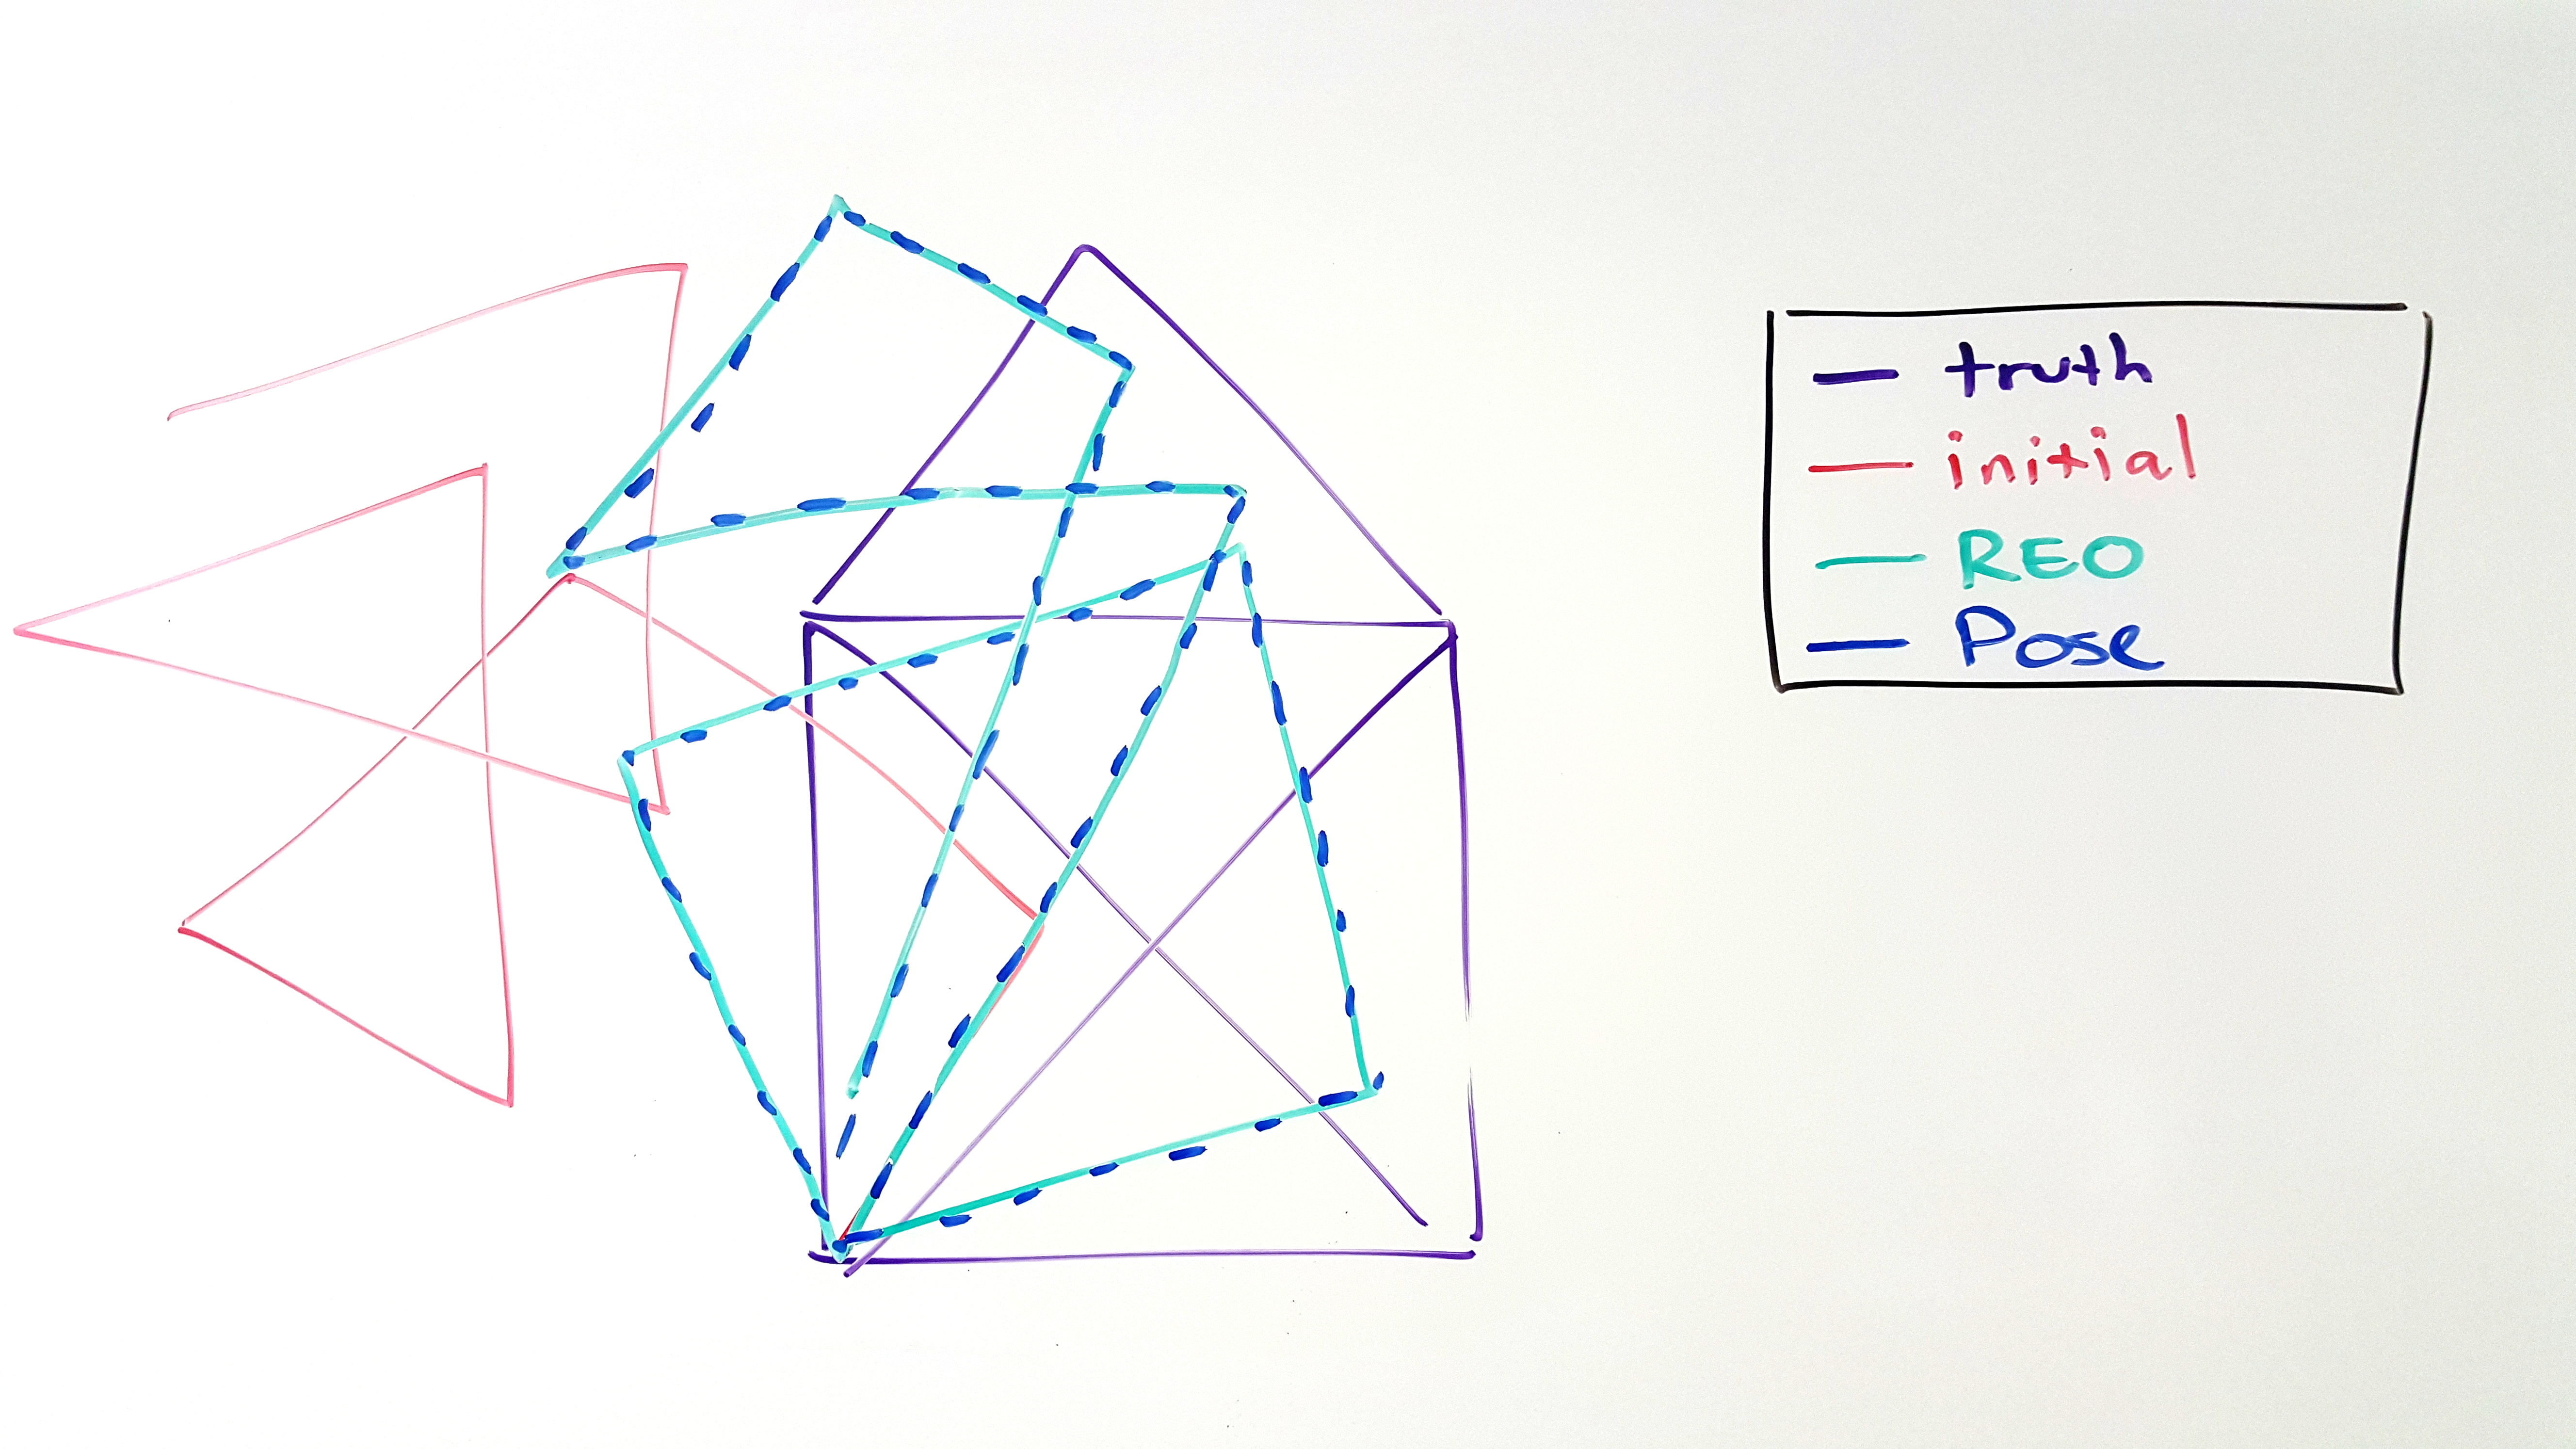
\includegraphics[width=0.7\textwidth]{figures/house_trajectory.jpg}
  \caption{One sample from a house trajectory with optimization results from relative edge optimization and global pose optimization}
  \label{fig:house_trajectory}
\end{figure}

\begin{figure}
  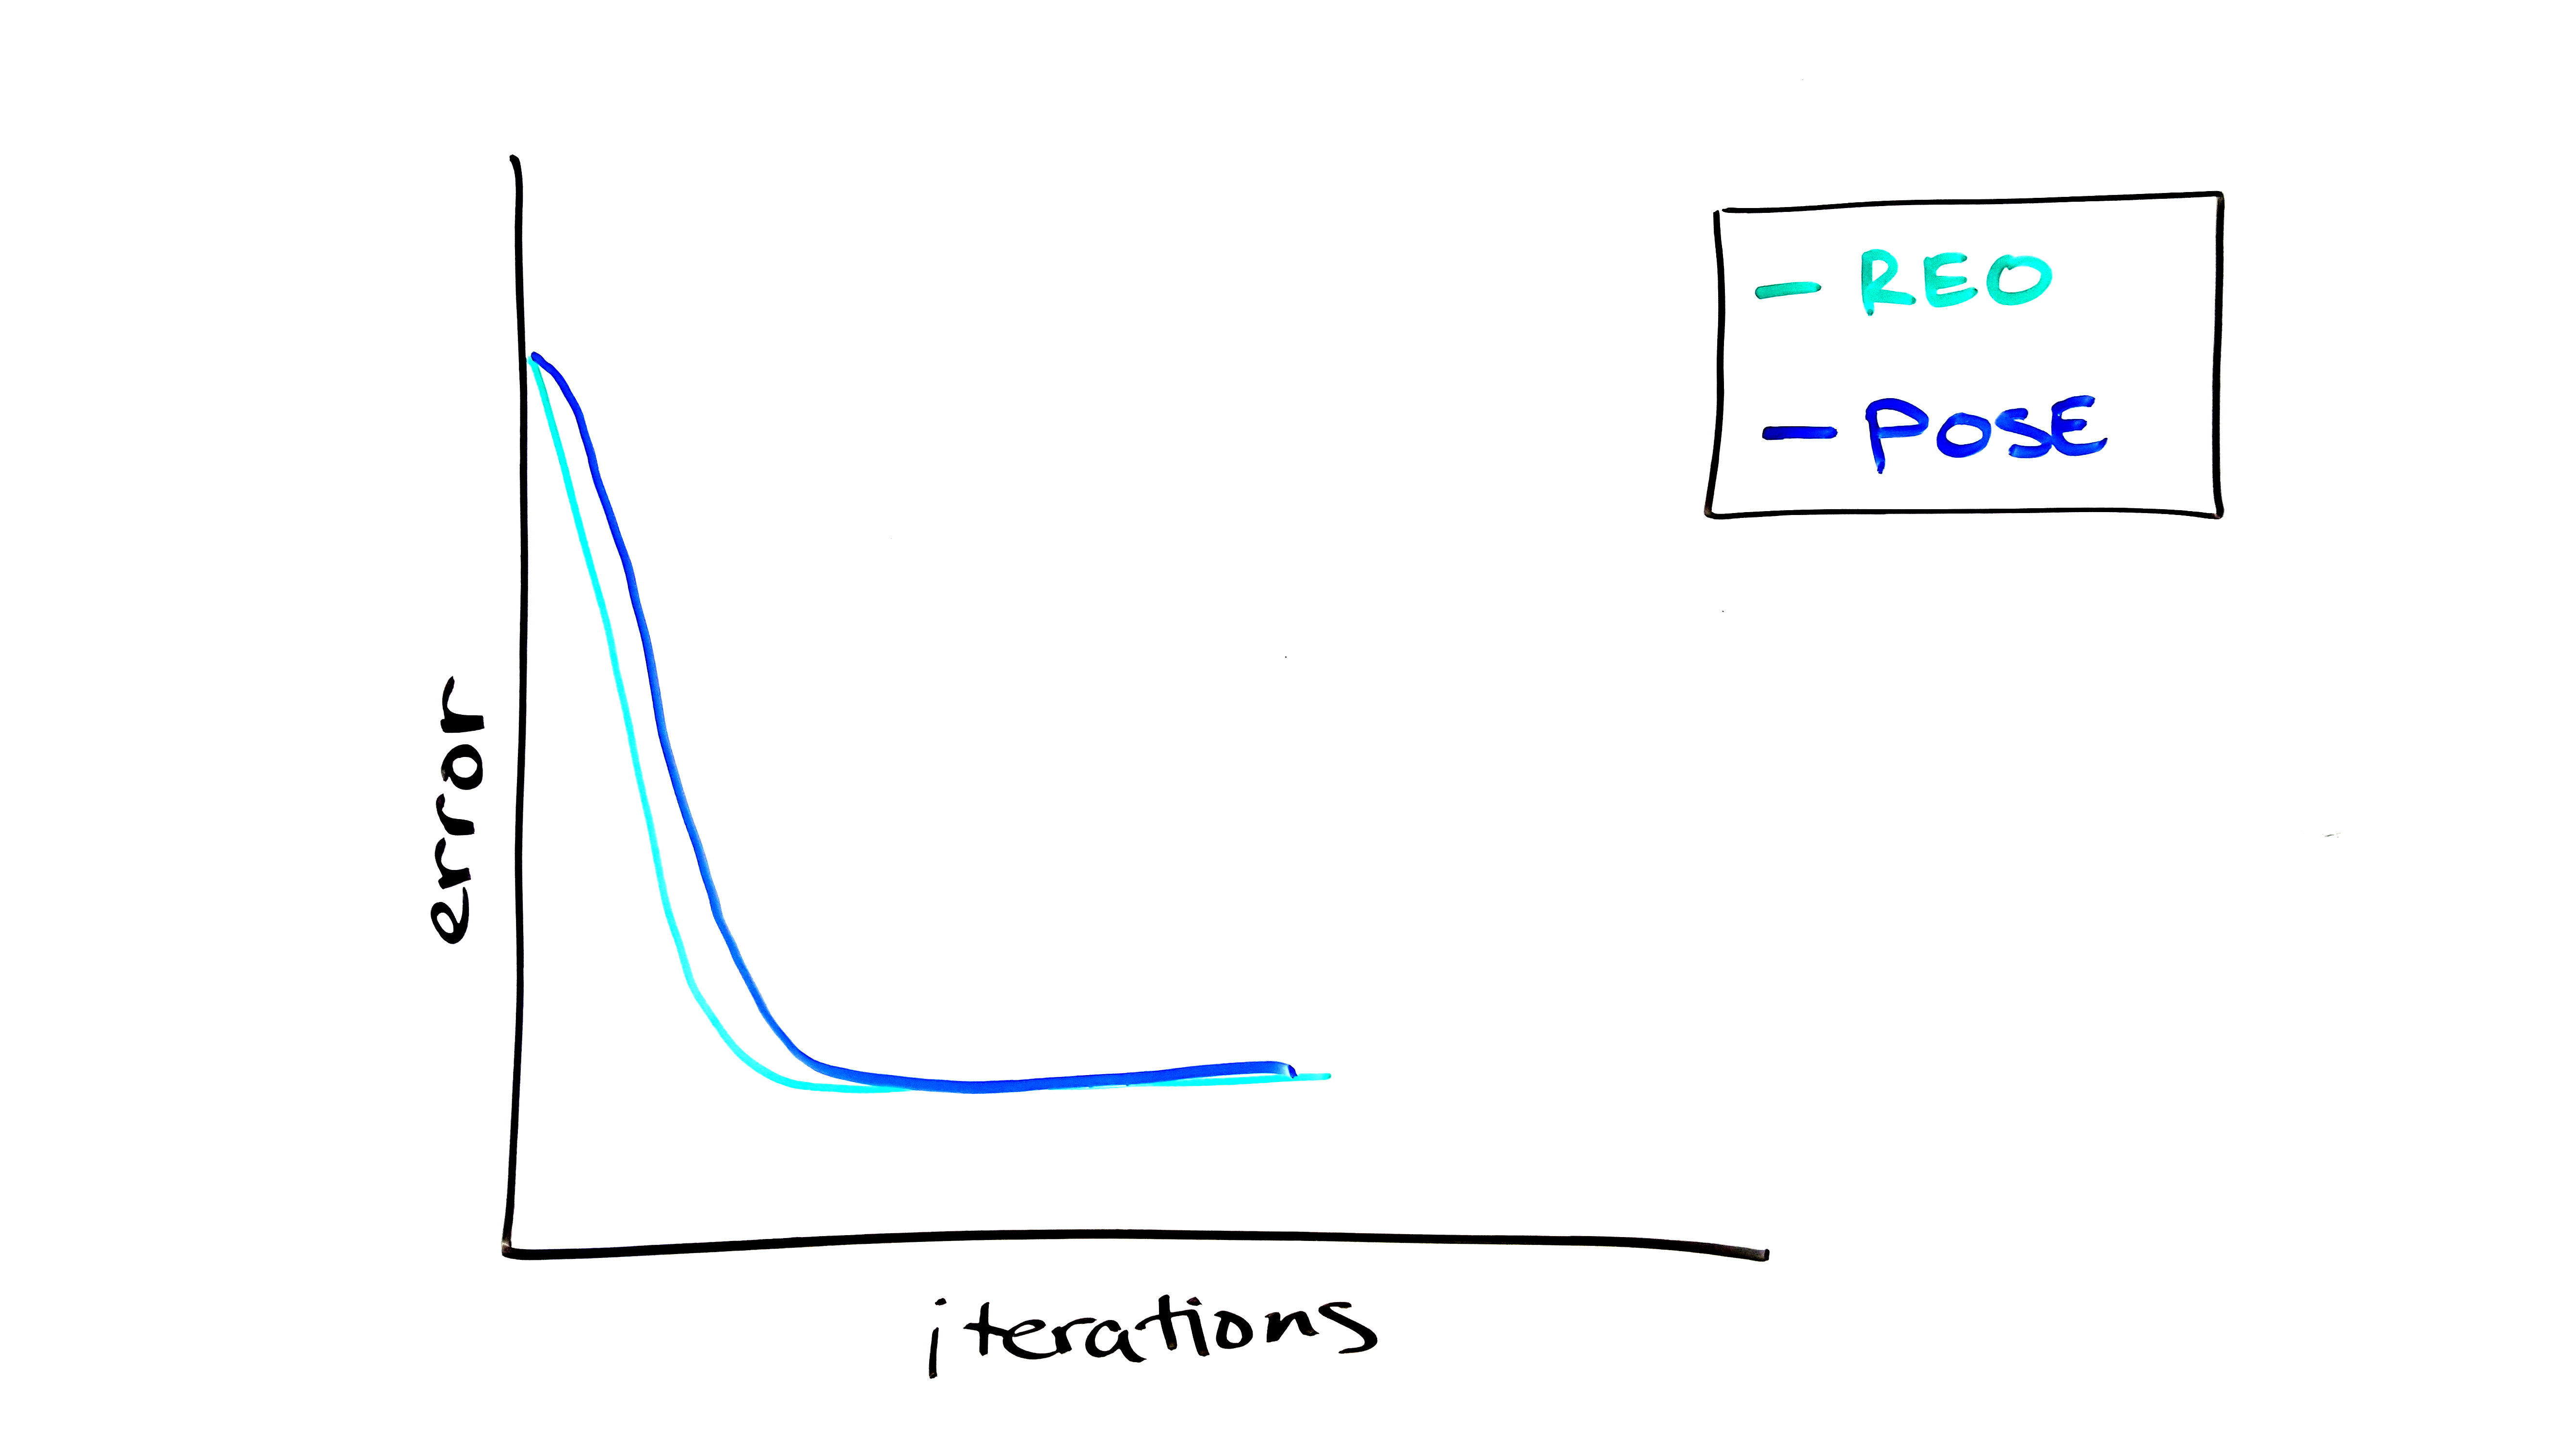
\includegraphics[width=0.7\textwidth]{figures/convergence_comparison_house.jpg}
  \caption{Convergence for the house trajectory}
  \label{fig:convergence_house}
\end{figure}

% show that they are equivalent
It can be plainly observed from comparing Eq~\ref{eqn:global_opt} and Eq~\ref{eq:relative_opt} that relative edge optimization simply parametertizes the same cost function with relative edge constraints as opposed to global constraints, and therefore should result in an equivalent solution.  However, due to the different linearization between the two parameterizations, a simulation study was performed to show the equivalence of global pose and edge-based optimization. This was performed by optimization a house-shaped trajectory, shown in Figure~\ref{fig:house_trajectory} which was corrupted with random gaussian noise, had a random selction of edges were reversed and a loop closure placed between nodes at the bottom left corner of the trajectory. Every one of these optimizations produced identical results between global pose and edge-based optimization with a comparable number of iterations, shown in Figure~\ref{fig:convergence_house}.

% describe differences (pros/cons)
Differences between the performance of global pose graph and relative edge-based optimizations can be observed by exercising linearization errors.  For example, if the house trajectory is initialized with a 180$^\circ$ heading error, and provided global measurements, the global pose optimization often struggles to find the global minimum.  A similar experiment with 10,000 house trajectories was performed, except with the addition of a global measurement located at the peak of the house.  In this study, the pose graph optimization failed to converge to the correct optimum (As shown in Figure~\ref{fig:g2o_heading_divergence}) $20\%$ of the time, came to the same result but took more iterations as relative edge optimization $50\%$ of the time, and performed equivalently (same number of iterations, same result) the remaining $30\%$ of the time.

\begin{figure}[H]
  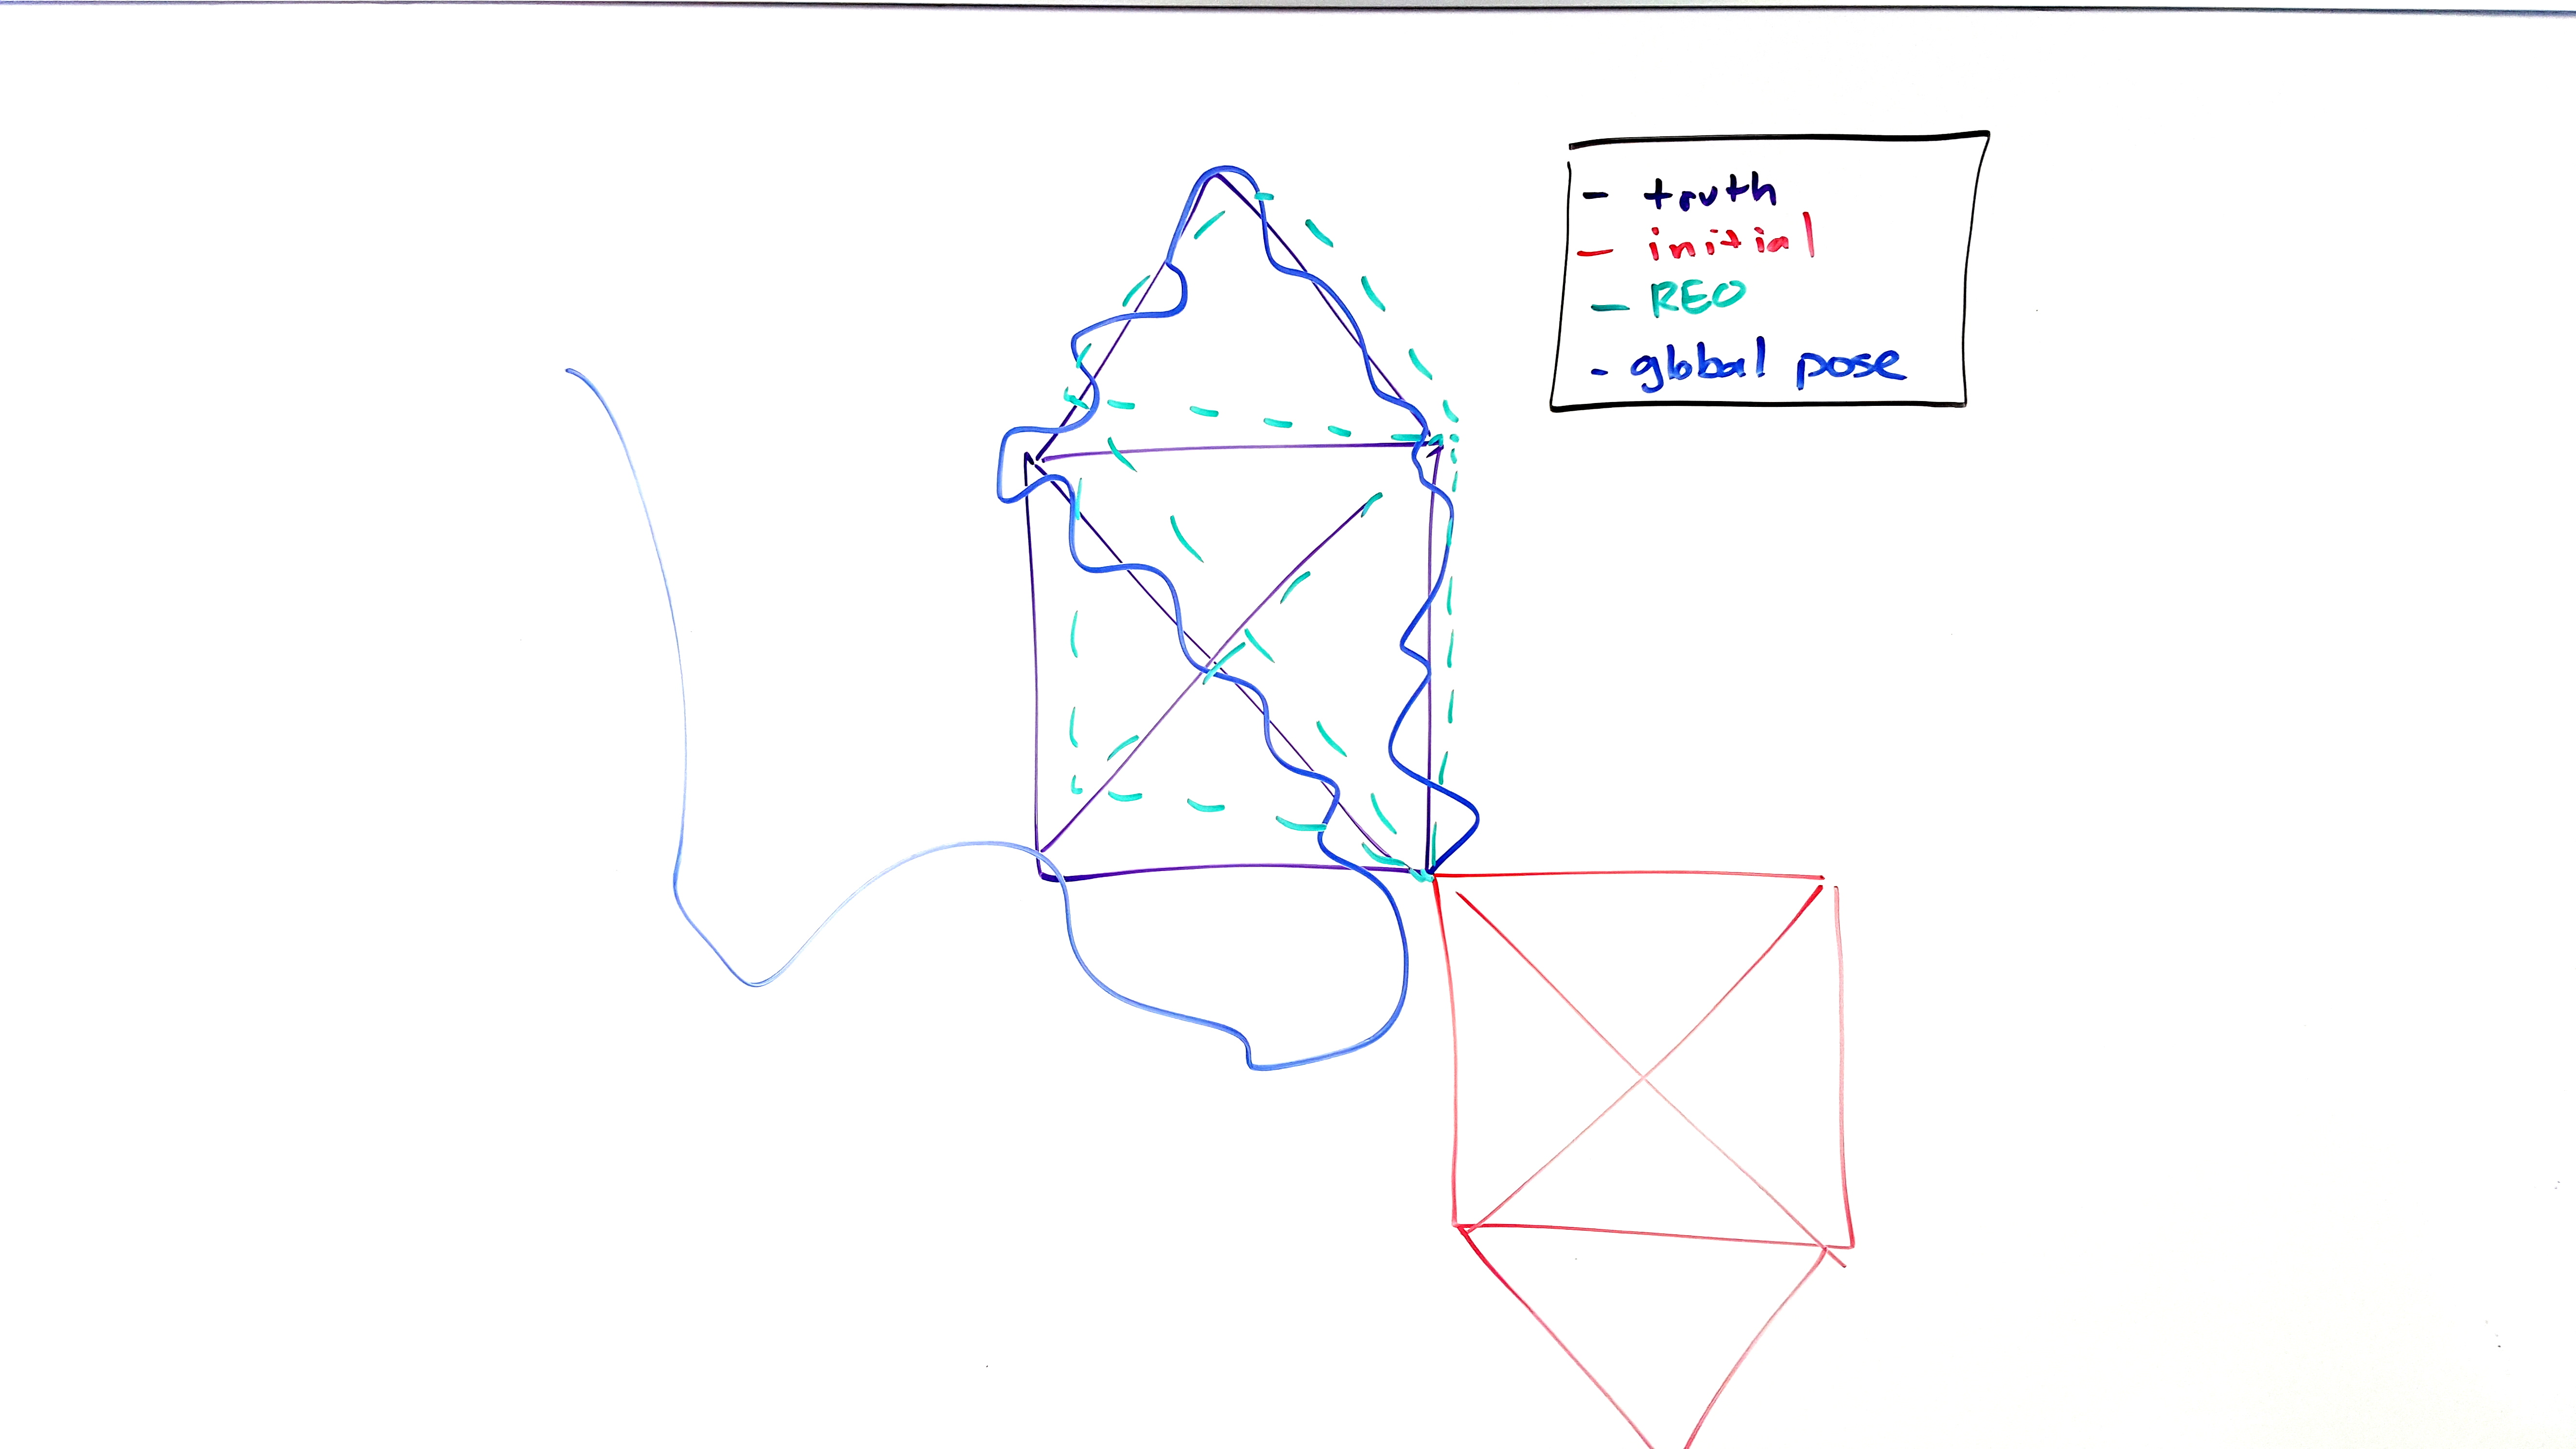
\includegraphics[width=0.7\textwidth]{figures/house_g2o_diverged.jpg}
  \caption{One sample from simulation study with a single global measurement added to peak of house trajectory,  initialized with a 180$^\circ$ heading error.  In this simulation, the global pose optimization failed to find the correct optimum.}
  \label{fig:g2o_heading_divergence}
\end{figure}

While relative edge optimization promises significant improvements in dealing with initialization errors when compared with global pose optimization, it is not as easily scaleable as global pose graph optimization.  In particular, the calculation of $\frac {\partial\Delta t_{a-z}}{\partial\Delta t_{ij}}$ causes significant correlations between edge estimates in a loop closure.  This ultimately leads to a loss of sparsity in the calculation of $\mathbf{H}_{az}^\top \Omega_{az} \mathbf{H}_{az}$ in Equation~\ref{eqn:3d_opt}.  The parameterization of global pose optimization however, does not run into this issue and can therefore exploit sparsity in solving for $\Delta \mathbf{x}$.  This becomes most important when considering a loop closure with a large number of edges where a dense matrix solve can be very costly. Secondly, in typical pose graph implementation, the number of edges can grow explosively if an agent repeatedly navigates the same area.  In this situation, the sum in the second term of the cost function in Equation~\ref{eqn:cost_function} can become extremely large and costly to calculate.


% how to use them together
To overcome these issue, we propose a two-fold solution.  To reduce the number of terms summed in the second term of Equation~\ref{eqn:cost_function}, we propose stochastically iterating over smaller loop closures in a well-connected pose graph and optimizing only a selection at a time.  To reduce the size of the optimization, we will exploit the relative nature of edge-based optimization to recursively break the full optimization into small, easy-to-manage problems.  This recurisve process has the added benefit of producing a completely parallelizeable independent computations which can be distributed to a GPU for fast evaluation.  While these solutions improve the scaleability of edge optimization, it still does not compete with the state-of-the-art global pose graph optimization libraries in terms of speed.  Due to the different parameterization, however, it can quickly bring a poorly initialized graph into a region where global pose graph optimization can quickly converge to a solution.  Therefore, we propose that edge optimization be performed for just a few iterations in situations where global pose graphs may struggle to find global minima to initialize the graph.  After much of the error has been removed by the more expensive, but less sensitive edge optimization, global pose graph optimization can very quickly find a global minima even in highly-connected and complicated graphs, where repeated edge optimization may become intractable.
